\documentclass[sigconf]{acmart}
\setcopyright{none}
\settopmatter{printacmref=false,printccs=false,printfolios=true}
\renewcommand\footnotetextcopyrightpermission[1]{}
\acmConference[SymDiv]{Source-Verified C Analysis}{2026}{Online}
\acmYear{2026}
\copyrightyear{2026}
\usepackage{booktabs}
\usepackage{listings}
\usepackage{graphicx}
\usepackage{xcolor}
\emergencystretch=3em
\raggedbottom
\lstset{language=C,basicstyle=\ttfamily\footnotesize,columns=fullflexible,keepspaces=true,breaklines=true,frame=single,showstringspaces=false}
\newcommand{\VFourAbstract}{On 55 programs, LLM-guided search confirms 9/9 historical and 6/6 authored stress positives under a 128-operation budget; SMT lookahead confirms 9/9 and 5/6, respectively. Both find 11/19 external positives. In 75 fresh timing trials on five preselected programs, Local-first reduces model requests from 15 to 9 per 15 trials without lowering the pooled median time. A later exploratory SMT-first extension uses 3 requests with unchanged discovery on the same programs. }
\newcommand{\VFourResource}{The strongest symbolic control substantially narrows the gain over DFS (Table~\ref{tab:v4-main}). On historical diagnostics, SMT lookahead and LLM-guided search both confirm 9/9 positives, compared with 5/9 for DFS and 4/9 for Portfolio. On authored stress programs, LLM-guided search confirms 6/6, SMT lookahead 5/6, and DFS 0/6. Resource-selective Local-first also confirms 6/6, with its prepass charged to the shared budget. Figure~\ref{fig:v4-budget} shows all three budget settings: the difference between SMT lookahead and LLM-guided search closes at 512 operations. LLM-guided search produces 0 false positives across the three cohorts; its negative outcomes still distinguish complete refutation from unknown.}
\newcommand{\VFourLoopCase}{The remaining main-budget difference is explained by s011, an eight-iteration weighted loop. LLM-guided search reaches its witness in 78 state pops. SMT lookahead first spends 61 summary-node visits; the combined search requires 139 charged operations and exceeds the 128-operation limit. The 512-operation run confirms the same defect. Thus the extra main-budget discovery depends on charging advice construction, rather than on a defect uniquely accessible to the LLM.}
\newcommand{\VFourExternal}{LLM-guided search and SMT lookahead each confirm 11/19 external positives, while CSA warns on 12/19 (Table~\ref{tab:v4-main}). The guided result includes 5/6 complete refutations on negative programs and 9 unknowns overall. The eight missed positives involve wider integer types (four), mutable globals (two), expression side effects (one), and generic selection (one). The remaining unknown is a negative program using unsupported \texttt{sizeof}. Every selected program remains in the denominator. The flat external curves in Figure~\ref{fig:v4-budget} show that increasing the operation budget does not overcome these semantic limitations.}
\newcommand{\VFourFeedback}{Exactly 1 natural correction event is observed, on the reused historical response for d005. Its source verification failure occurs at state pop 51, after the old fixed 48-pop probe. The model had incorrectly claimed that $2\times5-11=0$. A fresh request changes the unverified site verdict from \texttt{bug} to \texttt{safe}, at a cost of 11.05\,s. The final analyzer result remains \texttt{unknown}. Relative to the paired run without feedback, there are 0 additional positive discoveries and 0 lost discoveries. The corrected verdict therefore demonstrates a successful trigger, while the retained unexplored paths prevent a complete refutation.}
\newcommand{\VFourTiming}{Every main timing method confirms 9/9 positive runs, completely refutes 3/6 negative runs, and leaves three runs unknown (Table~\ref{tab:v4-timing}). Local-first uses 9 model requests instead of 15 for Always-request. Their medians across the 15 runs are 20.81\,s and 19.45\,s, respectively, compared with 0.24\,s for SMT lookahead. Request reduction therefore does not translate into a lower pooled median on this workload. Figure~\ref{fig:v4-case-time} shows why: the local gate avoids remote waiting on c010 and c013, but the harder positive programs still take much longer than SMT lookahead. All methods reach the 30\,s deadline on the unresolved negative s008. Each plotted point includes preparation and provider waiting; no recorded service time is subtracted. The corrected main cohort contains 0 provider failures. The pooled medians describe these selected programs, not a general speedup estimate.}
\newcommand{\VFourExtension}{The strength of SMT lookahead motivates running it before the Local-first request gate. This integration is frozen and evaluated after the main study, using three fresh trials on each of the same five programs and the unchanged 30\,s allowance. It confirms 9/9 positive runs, completely refutes 3/6 negative runs, and uses 3 requests; its pooled median is 0.23\,s. Figures~\ref{fig:v4-case-time} and~\ref{fig:v4-calls} mark this later arm separately. SMT lookahead already produces all positive discoveries; the remaining requests occur on s008 and add none. The extension implements a cost-motivated workflow, but its later, non-interleaved comparison on already studied programs is exploratory rather than held-out evidence.}
\newcommand{\VFourVariance}{Re-evaluating the three fresh Always-request responses under the fixed operation budget changes the warning/result pair for 0/5 programs and the state-pop count for 0/5. Three repetitions remain a limited probe of response variability. The complete experimental ledger contains 74 new request attempts: 38 for the resource study, 8 for the invalid-clock cohort, 24 for corrected timing, 3 for SMT-first, and 1 for the source-location repair. They account for 1,368,439 known tokens and 1110.35\,s of recorded provider time. Usage is incomplete for 1 request, so the token total is a lower bound. Reused historical responses are not counted as new requests; invalid attempts remain included in the expense.}
\newcommand{\VFourValidation}{All 101 distinct accepted witnesses in the primary resource and fresh-timing records are confirmed by compiled C/UBSan at the expected source lines, covering 809 repeated finding occurrences. All 19 external positive labels also have independent compiled witnesses, including programs outside the interpreter's support. The regression suite passes 112 tests. These checks support accepted positives and implementation invariants; they do not prove the source model or every negative label.}
\newcommand{\VFourSiteRepair}{A final audit exposed an interface defect on c008: the nested divisions in \texttt{x/2*3/0} share an AST range beginning. The old catalog merged their identities, omitted the zero divisor from the model's site list, and attached the wrong denominator metadata to a real file-level finding. Line-level UBSan validation could not distinguish the operators. The repair uses distinct operator tokens when ranges collide, shared by extraction and both symbolic engines. Only c008 changes in an audit of all 55 catalogs; its separate fresh response reports the defect. The frozen LLM-only result remains 16/19, including this interface-induced miss. The repaired location passes a line-and-column UBSan check. Reruns at all three budgets and 110 current main-budget DFS/LLM-guided comparisons show 0 warning/result differences. The fresh request and repair are recorded separately. Archived replay uses the original catalog mapping; ordinary analysis uses the corrected mapping.}
\newcommand{\VFourReproduction}{Completed offline regeneration reproduces all 37 new sources byte for byte and makes 0 model requests. Every fixed-budget warning/result pair matches the recorded result. It also confirms 88 distinct replay witnesses in compiled C.}
\newcommand{\VFourConclusion}{At the main operation budget, SMT lookahead matches LLM-guided search on the 9/9 historical discoveries and finds 5/6 stress positives versus 6/6. That difference disappears with a larger operation budget, while external failures persist. Local-first reduces timing requests from 15 to 9 without a lower pooled median. The later SMT-first extension uses 3 requests on the same workload, with no additional discovery from those remaining calls. }

\title[SymDiv: LLM Guidance under Resource Budgets]{SymDiv: Evaluating LLM Guidance for Source-Verified Division-by-Zero Detection}
\author{SymDiv Project}


\begin{document}
\begin{abstract}
Large language models (LLMs) can propose paths to a defect, but useful advice
must remain valid under source semantics and justify its own cost. We present
SymDiv, a source-verified analyzer for integer division and remainder by zero
in C. The LLM supplies branch preferences to a retained symbolic frontier;
source-derived constraints determine whether an input is a confirmed witness.
We compare this design with Clang Static Analyzer and same-engine search
policies, including a control based on satisfiability modulo theories (SMT).
\VFourAbstract{}
The study shows that the apparent value of LLM guidance depends on the
strength of the symbolic control, the accounting of advice construction,
and the distinction between request reduction and end-to-end time.
\end{abstract}
\begin{teaserfigure}
\centering
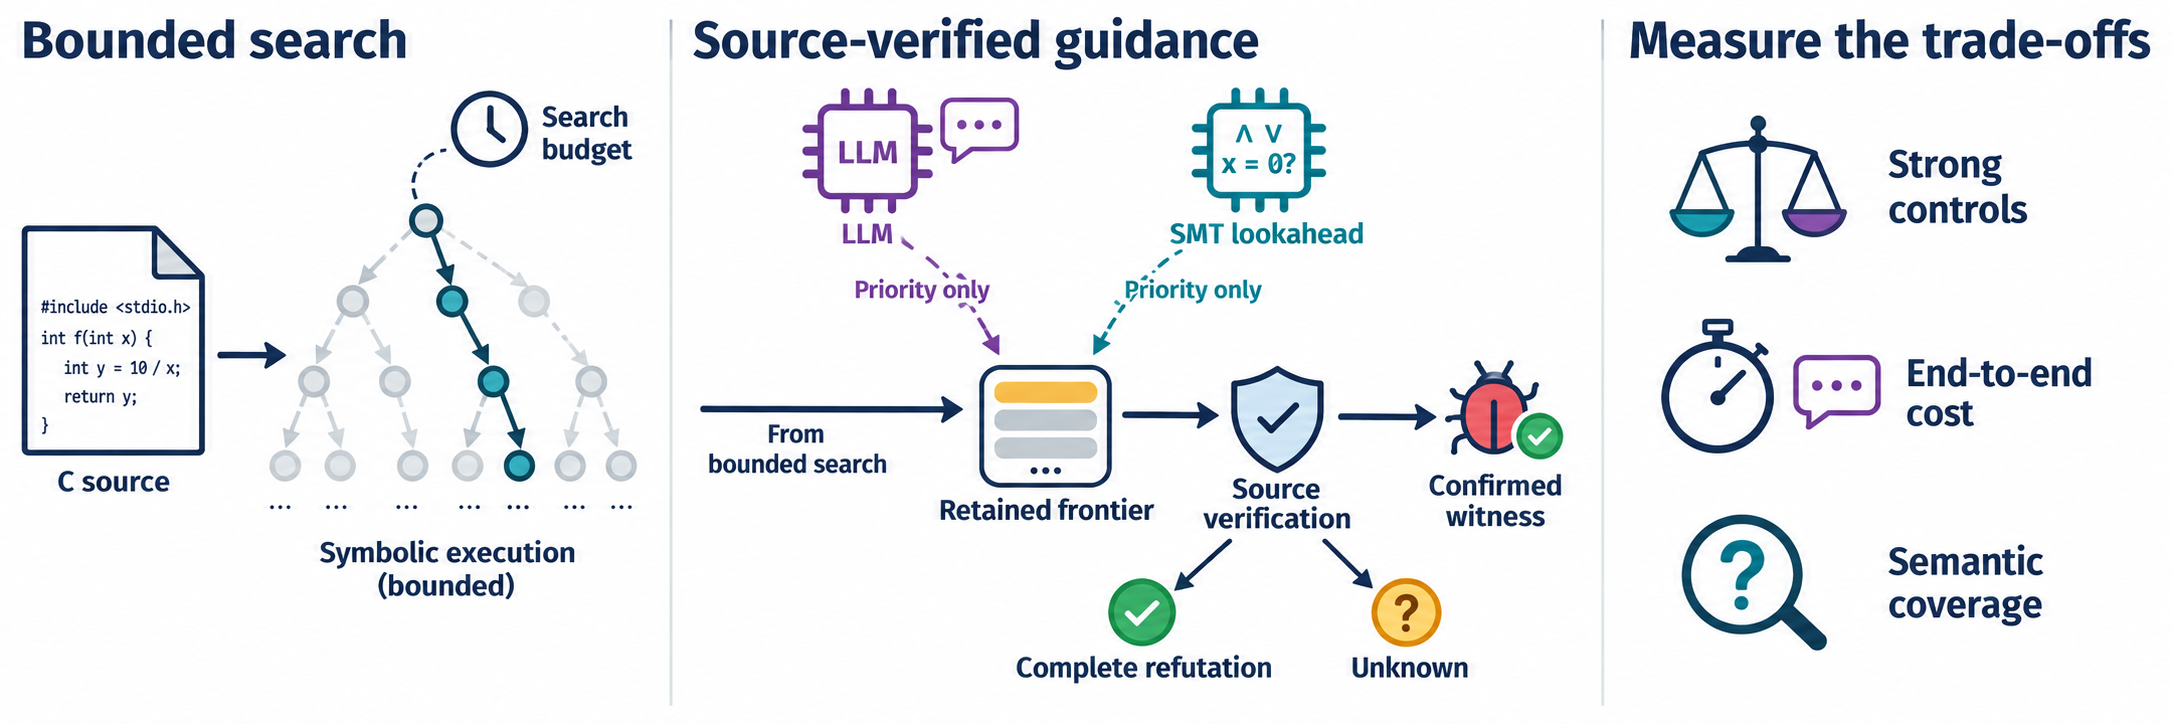
\includegraphics[width=\textwidth]{figures/v4/teaser.png}
\caption{SymDiv separates search guidance from source verification. LLM branch
preferences and SMT lookahead prioritize the retained frontier; source-derived
constraints determine acceptance. The evaluation measures bounded discovery,
end-to-end cost and semantic coverage. GPT-Image generated this conceptual
illustration; Figures~\ref{fig:v4-budget}--\ref{fig:v4-calls} report measured data.}
\Description{A conceptual overview of bounded path exploration, alternative
LLM and SMT guidance, a retained frontier, source verification and explicit
outcomes. The three evaluation dimensions are strong controls, end-to-end
cost and semantic coverage. No experimental values are depicted.}
\label{fig:teaser}
\end{teaserfigure}
\maketitle

\section{Introduction}
An LLM can suggest a promising execution path without being trusted to decide
whether that path is feasible. This separation motivates LLM-guided symbolic
execution: a learned component directs exploration, while source semantics
and a solver determine whether a defect is reachable. Recent systems use LLMs
for path reasoning, search prioritization and harness synthesis
\cite{autobug,kleecopilot,sailor}. Their different integration points raise a
common evaluation question: which part of the analysis benefits from the LLM,
and does that benefit survive comparison with inexpensive symbolic reasoning?

This paper studies that question through integer division and remainder by
zero in C. The task has an explicit acceptance condition, yet branching and
bounded loops make discovery sensitive to search order. We implement SymDiv,
a symbolic interpreter built around Clang's parser and Z3. Its LLM interface
returns occurrence-indexed branch preferences. Those preferences affect only
the order in which pending states are explored; assignments, path constraints,
and witness acceptance remain source-derived. Alternative paths and spent
budgets persist across guidance, feedback and fallback phases.

A comparison against depth-first search (DFS) alone is insufficient to
attribute a discovery gain to learned reasoning. A more targeted symbolic
control may supply the same useful preferences. Likewise, a reduction in
state exploration may not compensate for a remote model request. We therefore
compare LLM-guided search with a shared-frontier portfolio and a bounded
SMT lookahead control, and evaluate operation budgets separately from actual
end-to-end time. Clang Static Analyzer (CSA) provides the external traditional
baseline on the same source files.

The study separates 18 historical diagnostics, 25 unchanged external Cppcheck
regressions and 12 authored stress programs. SMT lookahead matches the
historical discovery count of LLM-guided search, and the remaining stress-case
gap depends on the operation budget. Fresh timing on five preselected programs
shows that selective requests reduce model invocations without improving the
pooled median time. External misses expose unsupported source semantics.
These findings motivate a separately evaluated SMT-first extension.

The contributions are:
\begin{itemize}
\item A source-verified LLM-guided analyzer with a validated branch-preference
interface, a retained frontier, and one event-triggered correction.
\item A controlled evaluation that separates external warning behavior,
same-engine search policies, operation budgets, fresh timing and concrete
witness validation, with unsupported cases retained in the denominator.
\item An analysis of when guidance changes bounded discovery and when its
cost dominates, together with a separately frozen SMT-first extension and
an artifact preserving successful, negative and invalidated observations.
\end{itemize}
LLM-guided path prioritization is established prior work; this exploratory
study evaluates SymDiv's particular interface, controls and cost accounting.

\section{Analysis Contract and Baseline}
\label{sec:contract}
\subsection{Target property and result categories}
For a function-entry input $x$, a path $\pi$, and an integer division or
remainder site $s$, let $C_\pi(x)$ contain the source-derived path constraints
and definedness guards, and let $d_s(x)$ be the denominator at that site.
A confirmed witness satisfies
\begin{equation}
  \exists x,\pi:\ C_\pi(x)\ \land\ d_s(x)=0.
  \label{eq:acceptance}
\end{equation}
Earlier arithmetic must remain defined along the path: an earlier zero
denominator or signed overflow cannot justify a later finding. The evaluation
asks whether a file contains any reachable target defect, so the analyzer
reports at most one confirmed witness per file. Compiled C validation with the UndefinedBehaviorSanitizer (UBSan)
is a separate check on accepted inputs, described in Section~\ref{sec:validation}.

We use three result categories consistently. A \emph{confirmed witness} is
an input accepted by source verification. A \emph{complete refutation}
excludes the target defect after exhaustive exploration within the supported
source model. An \emph{unknown} result means that no witness was confirmed
and exploration is incomplete. Unsupported operations, exhausted budgets,
a final solver timeout, or a reachable continuation beyond the loop bound
produce unknown unless another path supplies a witness. In particular, a
negative warning classification is not necessarily a complete refutation.
Benchmark labels (bug/safe) and unverified LLM verdicts are kept separate
from these analyzer outcomes.

\subsection{Supported source and environment semantics}
The interpreter supports scalar 32-bit \texttt{int} and \texttt{unsigned int},
local assignment and lexical shadowing, integer arithmetic and comparisons,
short-circuit and conditional expressions, \texttt{if}, bounded
\texttt{for}/\texttt{while}/\texttt{do} loops, and return/break/continue.
Signed division truncates toward zero; signed remainder follows the sign
of the dividend. Unsigned arithmetic wraps modulo $2^{32}$. Signed-overflow
paths and the \texttt{INT\_MIN/-1} continuation are excluded under the declared
C model \cite{c11}. Loops admit at most eight iterations; hitting the bound
with a feasible continuation preserves incompleteness.

Each \texttt{rand()} call supplies an independent symbolic integer in
$[0,2^{31}-1]$. This environment abstraction does not model a particular
seeded generator. Declared void printing functions are observational.
Arbitrary calls, pointer memory, mutable globals, unsupported integer types
and uninitialized reads cause incompleteness. Analysis begins at each
function containing a target site, so reachability is relative to its entry
inputs rather than a whole-program calling context.

\subsection{Clang Static Analyzer}
CSA is a path-sensitive static analyzer whose checkers operate over symbolic
program states. We invoke its command-line analyzer on the same C files with
C11, the \texttt{core.DivideZero} checker and SARIF output
\cite{clang-checkers,clang-cli}. The artifact records commands, compiler
version, diagnostics, completion status and time. A successful process and a
readable report are required before a run is scored.

CSA's warning policy differs from our existential input contract. A possibly
zero parameter or random result need not receive the warning emitted for a
definitely zero denominator. A missing warning counts as a false negative
under the benchmark labels, but does not by itself isolate an advantage of
LLM guidance. Same-engine controls therefore share SymDiv's source model,
witness query and verification procedure, varying the search policy.

\section{Source-Verified Search Guidance}
\label{sec:method}
\subsection{Design rationale}
Two earlier designs clarify the role of guidance. The initial prototype
(version 1) accepted LLM-generated predicates without checking their
correspondence to the source. For
\texttt{if(x==0) return 0; return 42/x;}, omitting the early return admits the
spurious candidate $x=0$. A satisfiable explanation is insufficient when
its translation of the program is wrong.

Version 2 constructed source-feasible states before consulting the LLM.
If $S=C_\pi\land d_s=0$ and $H$ is an additional model predicate, then
$\mathrm{models}(S\land H)\subseteq\mathrm{models}(S)$.
After complete exploration, adding $H$ cannot introduce another real defect.
It may change solver difficulty, but this design measured no such benefit:
the hybrid and symbolic-only variants had identical warning classifications
on 48 small subjects. Their unchanged results, including the two negative
abstentions of the symbolic-only pilot, remain in the artifact.

The resulting design moves the LLM before exploration and restricts it to
priority advice. Version 3 established this retained-frontier interface;
version 4 is the main study reported here. These version identifiers name
archived snapshots, rather than different semantic models within a comparison.

\subsection{Branch preferences and the retained frontier}
Clang produces a JSON abstract syntax tree (AST). The frontend assigns each
branch a stable identifier from the source hash, function, byte offset and
branch kind. The LLM receives the source, arithmetic-site catalog and branch
catalog, without benchmark labels or baseline predictions. Structured output
contains unverified site verdicts and \texttt{(branch\_id, visit, take)} tuples.
A \emph{branch preference} selects a branch direction at a particular loop
visit. Malformed identifiers, duplicate tuples and non-Boolean directions
are rejected; the obsolete free-form predicate field must be empty.

A symbolic state contains the store, lexical bindings, path constraints,
inputs, decision trace and continuation frames. An \texttt{if} enqueues both
successors; loop frames retain both the exit alternative and iteration count.
The \emph{retained frontier} is this set of pending states. LLM-guided search
ranks a state by disagreements between its trace and the supplied preferences,
breaking ties by the most recently enqueued state. Unspecified decisions tie.
The actual branch condition is evaluated by the interpreter in every case.
Figure~\ref{fig:workflow} shows where this ordering policy enters the analyzer.

\begin{figure*}[t]
\centering
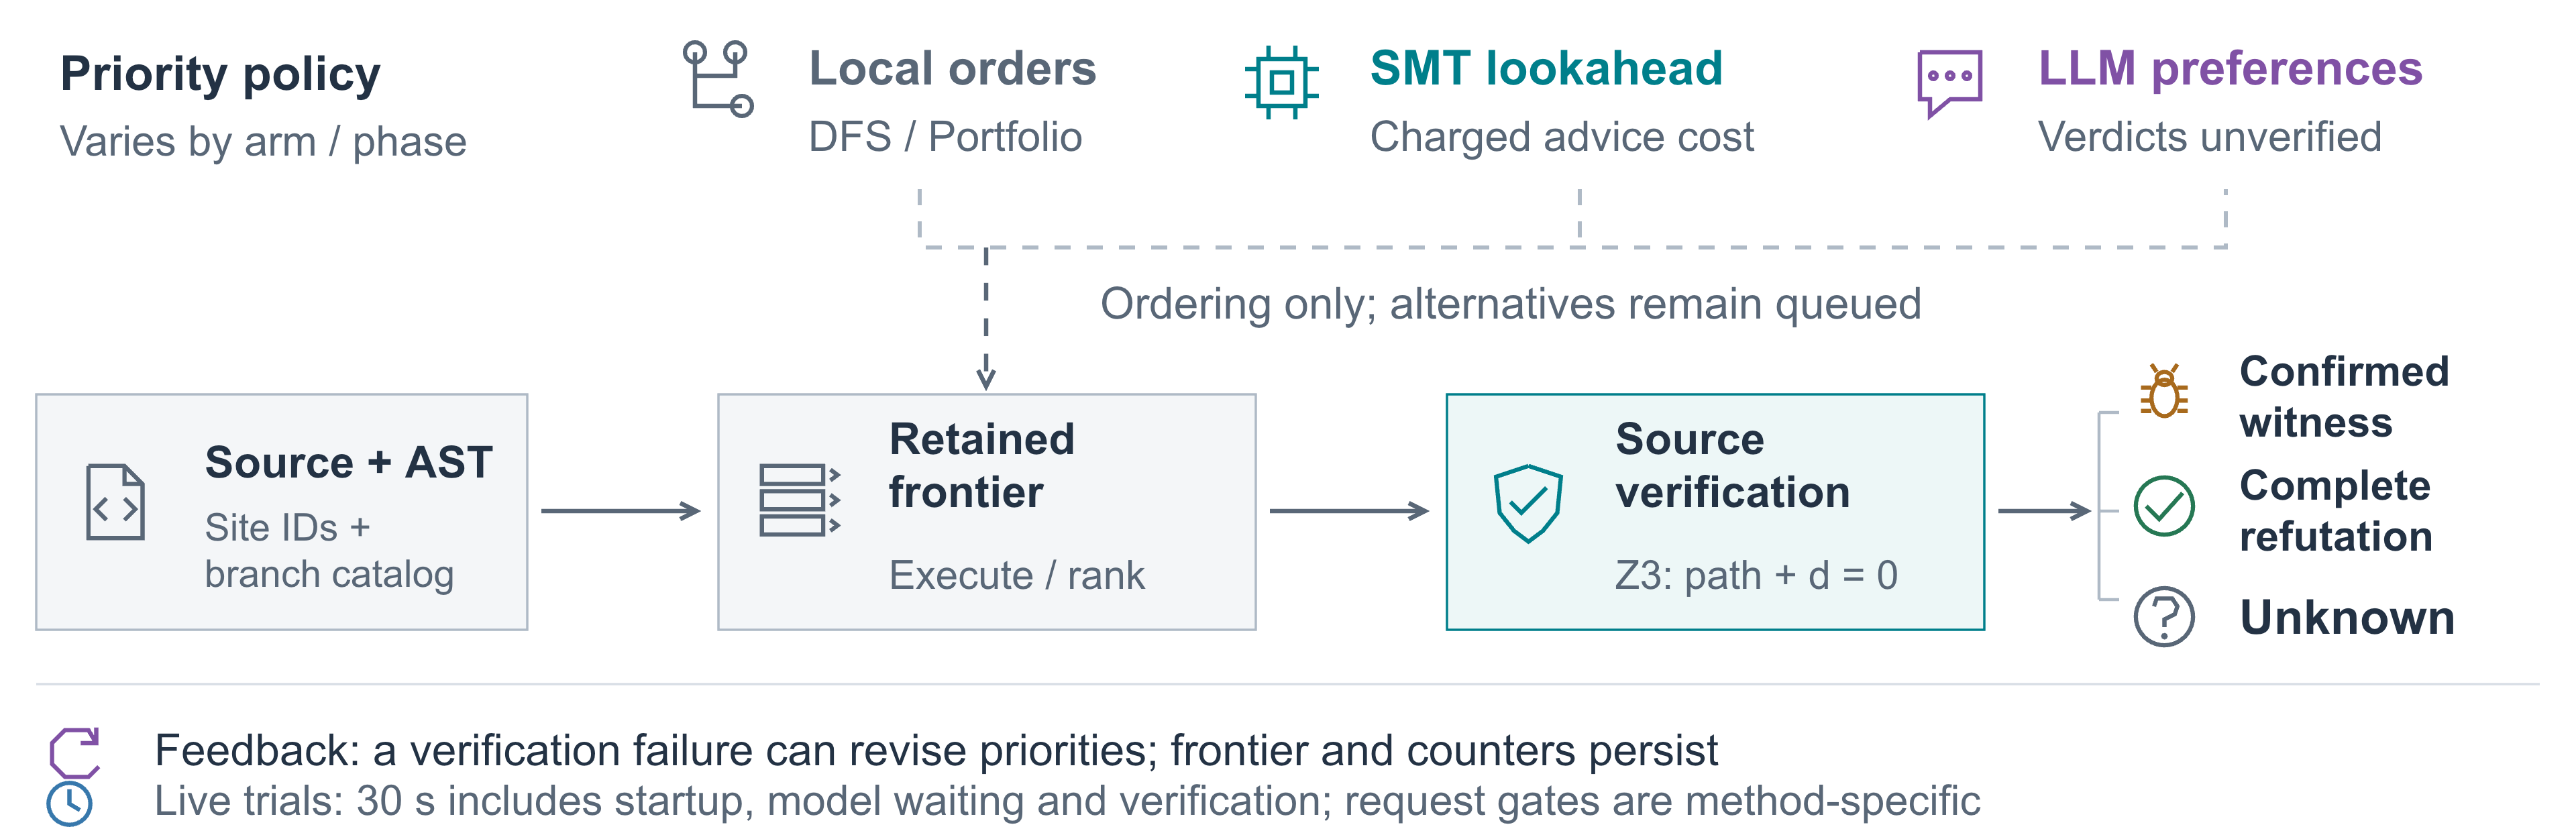
\includegraphics[width=\textwidth]{figures/v4/workflow.png}
\caption{SymDiv's retained-frontier architecture and policy alternatives.
Advice changes priority; only source-derived constraints, including definedness,
can accept a zero-denominator witness. Complete refutation requires exhausted
supported exploration; resource or semantic limits give unknown. One correction
is available only in the feedback arm. Live timing disables corrections.}
\Description{A compact diagram with labeled source, branch, chip, model, queue,
shield, bug, check, question, feedback and clock icons. Alternative local, SMT
and model policies feed only frontier priority. Source execution and Z3 checks
lead to a witness, complete refutation, or unknown.}
\label{fig:workflow}
\end{figure*}

At a target site, source verification checks Equation~\ref{eq:acceptance}.
A small fixed set of concrete input vectors first attempts exact substitution;
these attempts can confirm a witness but cannot establish complete refutation.
Otherwise Z3 solves the source-derived query \cite{z3}. Every search policy
uses the same candidate inputs and solver. Definitive UNSAT feasibility
results prune paths; feasibility timeouts retain them. A timed-out final
zero-denominator query records incompleteness. An LLM verdict of \texttt{safe}
never suppresses exploration.

Preferences can spend the budget on an unproductive path, but cannot directly
add a witness. Regression tests and concrete replay support this acceptance
boundary; they do not constitute a proof of the interpreter.

\subsection{Symbolic controls and budget accounting}
DFS, a syntactic heuristic and random priorities (seeds 11/29/47) provide
simple controls. Additional policies use branch-depth breadth-first order,
minimum-true or minimum-false discrepancy, least-visited-branch priority, and
optimistic AST statement distance to a target site. The \emph{Portfolio}
policy cycles distance/coverage/DFS/discrepancy every 16 state pops on the
same frontier. These are local implementations of search-policy families
also exposed by established engines \cite{klee-options}.

The stronger \emph{SMT lookahead} control merges scalar branch assignments
with if-then-else terms and unrolls simple bounded loops. It asks for a
zero-denominator candidate, translates that candidate into branch
preferences, and passes them to the same source interpreter. Advice
construction is limited to 64 summary-node visits (also at most half the
operation budget), 16 solver calls and one second. Unsupported summaries,
UNSAT results and timeouts do not prove safety or remove real paths.

We call the shared resource cap the \emph{operation budget}: each state pop
counts once, as does each summary-node visit for SMT lookahead. A state pop
processes a statement or continuation frame. Lookahead solver calls also
consume the separate \emph{solver-call budget}. These mixed operations are
an explicit accounting convention, not equal units of CPU work or CSA
nodes. Fresh end-to-end timing supplies the complementary cost comparison.

\subsection{Feedback and selective requests}
\label{sec:gates}
In the main resource experiment, LLM-guided search uses the initial
preferences for at most 80 state pops before Portfolio fallback. The
\emph{LLM-guided + feedback} variant may pause at the first failed source
verification event consistent with the encountered preferences of a
\texttt{bug}/\texttt{unknown} proposal. It requires a nonempty frontier and
at least 16 operations remaining. One fresh correction can reprioritize
that frontier for 32 pops; pending states and spent counters are preserved.
The trigger remains eligible after the initial guided phase.

Feedback includes the attempted trace, source failure and spent resources.
When available, an actual UNSAT core explains a failed zero-denominator
query; an unreachable branch is reported without inventing a core.
It contains no benchmark label or preferred answer. Paired runs share the
same initial response, and budget-sensitivity runs use initial responses
only, avoiding correction reuse under a different failure state.

\emph{Local-first} delays an LLM request until a local prepass leaves work
unresolved. The resource experiment charges 64 Portfolio pops before using
the recorded initial response. In fresh timing, the gate checks a two-second
local threshold at 16-pop boundaries and requires at least 12 seconds
remaining before issuing a request. \emph{Always-request} issues the initial
request without that prepass. Corrections are disabled in fresh timing to
isolate request gating. The later \emph{SMT-first} extension runs bounded SMT
lookahead before the Local-first gate; its evaluation is kept separate.

\section{Experimental Design}
\label{sec:experiment}
We organize the evaluation around four questions:
\begin{enumerate}
\item \textbf{RQ1---Bounded discovery:} Does LLM-guided search improve
confirmed discovery over strong same-engine controls?
\item \textbf{RQ2---External applicability:} How much of that behavior
extends to independently sourced regression programs?
\item \textbf{RQ3---Feedback:} Does correction after a natural source
verification failure improve discovery?
\item \textbf{RQ4---End-to-end cost:} Do guidance and selective requests
improve results once actual model latency is included?
\end{enumerate}

\subsection{Cohorts and ground truth}
Before the main comparative runs, commit \texttt{9028aaa} freezes code,
source hashes, labels, order, prompts and protocol. The three cohorts have
different roles and are never pooled into a production-wide accuracy score.

\paragraph{Historical diagnostics.}
The 18 existing mechanism diagnostics comprise independent branches,
correlated input bits and bounded random loops at depths 3/5/7, each with
a bug/safe pair. Positive denominators are $d-t$ for an attainable target;
negative mates use the odd integer $2d-(2t+1)$. Finite enumeration establishes
the constructed labels. These programs were inspected during development,
and their original initial LLM responses are reused.

\paragraph{External regressions.}
A deterministic extractor screens all 61 literal snippets in the
\texttt{zeroDiv*} methods of Cppcheck's pinned \texttt{testother.cpp}, excluding
the diagnostic-format test \cite{cppcheck-tests}. All 25 unchanged standalone
C11 snippets containing integer division are retained, including unsupported
syntax. Compiler failures and nonliteral checks are logged; original source,
license, commit and hashes accompany the artifact. The cohort has 19 positive
and six negative programs. These are regression snippets, not 25 production
projects or a random sample of C code.

Labels follow source behavior, independently of the expected upstream
warnings. Three snippets without an expected warning still admit a zero
denominator through function-entry inputs or static zero initialization.
Compiled witnesses independently confirm all 19 positive labels, including
unsupported cases. Negative-label arguments establish the relevant divisor
or conditional-evaluation property, without asserting absence of unrelated
undefined behavior. Public snippets may have appeared in model training.

\paragraph{Authored stress programs.}
Twelve new programs, generated with seed 20261001, use weighted sums,
shuffled correlated bits (depths 9/11) and affine-weight loops (depths 7/8).
Each setting has a positive and an odd-denominator negative mate; enumeration
establishes the attainable sums. These programs vary the diagnostic
structures and parameters but remain project-authored evidence. Their
selection precedes observed analyzer results. New external and stress
programs receive fresh initial LLM requests without labels or control results.

\subsection{Methods, settings and metrics}
The main operation/solver-call budgets are 128/256, with sensitivities of
64/128 and 512/1,024. The loop bound is eight. Final SMT queries allow
1,000\,ms; feasibility-pruning queries allow 25\,ms. CSA uses its native
configuration. The recorded environment is Python 3.9.6, Z3 4.13.3 and
Apple Clang 17 on macOS 26.1/arm64. LLM requests use Codex CLI with
\texttt{gpt-5.6-sol}, medium reasoning, structured output and no tools.
Codex supplies the provider interface; the analysis algorithm is independently
implemented in SymDiv.

LLM-guided, LLM-guided + feedback and the \emph{LLM-only} reference share
initial responses. LLM-only scores the unverified site verdicts, allowing
us to measure classification separately from source-verified discovery.
Resource-selective Local-first uses the same response only after its prepass.
Table~\ref{tab:v4-main} reports true positives (TP), false positives (FP),
complete refutations (S), and unknown results (U). CSA and LLM-only are
warning/verdict references; their negative classifications are not scored
as complete refutations. All policies and random seeds remain in the raw
artifact, including those omitted from the compact main table.

\begin{figure*}[t]
\centering
\includegraphics[width=\textwidth]{figures/v4/budget-sensitivity.pdf}
\caption{Budget sensitivity on three separately reported strata. The shaded
band marks the main 128-operation budget; solver-call budgets are twice the operation budgets.
Each panel uses its own positive denominator and count scale. Coincident curves
represent equal counts. The stress advantage over SMT lookahead closes at 512;
external discovery stays at 11/19. These are deterministic recorded counts,
not estimates with confidence intervals.}
\Description{Three line plots of confirmed positives at operation budgets 64, 128,
and 512. LLM-guided search yields 8,9,9 historical positives and 4,6,6 stress positives;
SMT lookahead yields 7,9,9 and 2,5,6. All four controls find 11 external positives
at every cap. DFS and portfolio remain below guidance on authored cases.}
\label{fig:v4-budget}
\end{figure*}

\subsection{Fresh timing and measurement correction}
Five programs are fixed before timing results: c010 (external safe loop),
c013 (external equality defect), s003 (weighted defect), s008 (correlated
safe program), and s011 (bounded-loop defect). Each receives three fresh
trials under DFS, Portfolio, SMT lookahead, Always-request and Local-first:
75 process trials in a fixed hash-permuted order. Every model invocation
makes a fresh request; responses are not cached for this comparison.

An external parent measures the 30\,s allowance from startup through source
preparation, provider waiting, parsing, search and result return. Requests
are limited by actual remaining time, and late results become unknown.
The initial attempt exposed incompatible \texttt{time.monotonic()} origins
across processes on the recorded macOS/Python runtime \cite{python-time}.
The entire 38-trial partial cohort, including a watchdog failure of at least
45\,s, is archived and excluded together. Its costs remain in the ledger.

Before collecting all 75 corrected trials, a hashed amendment introduces
shared POSIX \texttt{CLOCK\_MONOTONIC} timestamps, maps them into each worker's
local clock origin, and makes the parent enforce the original deadline on
the entire process group. Subjects, policies, repetitions, order and budgets
remain fixed. Cross-process and forced-interruption regressions validate
the correction. Resource experiments use a single process and are unaffected.

Every request attempt is logged before it starts, with no retries. The
ceiling is 80 attempts and a 1.8-million observed-token stopping threshold;
missing usage is recorded as incomplete. Each of the three Always-request
responses per program is also re-evaluated under the fixed operation budget
as a variability probe. Five selected programs and three repetitions support
descriptive comparisons, not a population-level significance claim.

\section{Results}
\label{sec:results}
\begin{table*}[t]
\centering\small
\caption{Main resource comparison (128 operations / 256 solver calls). Historical diagnostics, external Cppcheck regressions and authored stress remain separate. TP is confirmed bug discovery except for CSA/LLM-only reference classifications; S denotes complete refutation, U unknown. CSA has native budgets; LLM verdicts are not safety proofs.}
\label{tab:v4-main}
\begin{tabular}{lrrrrrrrrrrrr}\toprule
 & \multicolumn{4}{c}{Historical: 9 bug / 9 safe} & \multicolumn{4}{c}{External: 19 bug / 6 safe} & \multicolumn{4}{c}{Stress: 6 bug / 6 safe}\\
Method & TP & FP & S & U & TP & FP & S & U & TP & FP & S & U\\\midrule
Clang CSA & 7 & 0 & -- & -- & 12 & 0 & -- & -- & 4 & 0 & -- & --\\
DFS & 5 & 0 & 3 & 10 & 11 & 0 & 5 & 9 & 0 & 0 & 0 & 12\\
Portfolio & 4 & 0 & 3 & 11 & 11 & 0 & 5 & 9 & 0 & 0 & 0 & 12\\
SMT lookahead & 9 & 0 & 2 & 7 & 11 & 0 & 5 & 9 & 5 & 0 & 0 & 7\\
LLM-only & 9 & 1 & -- & -- & 16 & 0 & -- & -- & 6 & 0 & -- & --\\
LLM-guided & 9 & 0 & 3 & 6 & 11 & 0 & 5 & 9 & 6 & 0 & 0 & 6\\
LLM-guided + feedback & 9 & 0 & 3 & 6 & 11 & 0 & 5 & 9 & 6 & 0 & 0 & 6\\
Local-first & 9 & 0 & 3 & 6 & 11 & 0 & 5 & 9 & 6 & 0 & 0 & 6\\
\bottomrule\end{tabular}
\end{table*}
\begin{table}[t]\centering\small
\caption{Fresh end-to-end 30 s trials: five cases, three repetitions each (9 positive and 6 negative runs). Median times pool the fixed selected cases; no universal speedup is inferred.}
\label{tab:v4-timing}
\begin{tabular}{lrrrrr}\toprule
Method & TP & S & U & Calls & Median s\\\midrule
DFS & 9 & 3 & 3 & 0 & 21.08\\
Portfolio & 9 & 3 & 3 & 0 & 5.32\\
SMT lookahead & 9 & 3 & 3 & 0 & 0.24\\
Always-request & 9 & 3 & 3 & 15 & 19.45\\
Local-first & 9 & 3 & 3 & 9 & 20.81\\
\bottomrule\end{tabular}\end{table}

\subsection{RQ1: Strong controls narrow the discovery gain}
\VFourResource{}

\VFourLoopCase{}
The useful distinction is therefore between reaching a witness within a
particular accounting limit and solving a defect unavailable to symbolic
reasoning. The fresh timing experiment tests the cost of both advice sources.

\subsection{RQ2: External misses track semantic coverage}
\VFourExternal{}

A separate applicability screen uses one fixed translation unit from each
of libpng 1.6.44, libsndfile 1.2.2 and libtiff 4.7.0
\cite{libpng,libsndfile,libtiff}. They contain respectively 8/59/10 functions
with target sites and 23/59/31 integer arithmetic sites. Configuration and
AST compilation succeed after retaining and repairing an initial missing
libpng-generated-header failure. Every target-containing function requires
memory, non-scalar types or calls beyond the supported model; the restricted
frontend also rejects preprocessing directives. No function is manually
sliced to remove those requirements. This is a feasibility screen, not a
whole-library analysis or a ground-truth bug-detection benchmark.

\subsection{RQ3: Feedback corrects a verdict, not discovery}
\VFourFeedback{}

The observation supports the event-triggered implementation and the
separation of a model verdict from a source-verified outcome. One historical
failure is too little evidence to estimate a general recovery rate; the new
external and stress cohorts contain no qualifying natural correction event.

\begin{figure*}[t]
\centering
\includegraphics[width=\textwidth]{figures/v4/fresh-timing.pdf}
\caption{Actual end-to-end time for every fresh trial: five preselected cases,
three repetitions per method. Circles are individual trials and vertical ticks
are case medians on a logarithmic scale. Right-pointing triangles mark unknown
outcomes at the 30\,s deadline (including small supervisor overhead), not solved
cases. The five main rows contain 75 corrected trials. The shaded SMT-first*
row contains 15 later exploratory trials on the same programs; it is separate
from the main interleaved comparison. c010/c013 are external and s003/s008/s011
are authored stress cases.}
\Description{Five panels display all 90 timing observations. SMT lookahead
resolves each positive in less than one second, whereas Always-request on hard
positives takes roughly 20 to 26 seconds. Local-first gating avoids remote
waiting on the two easy external cases. Every s008 run ends unknown near 30
seconds. The later SMT-first extension is separated with shading.}
\label{fig:v4-case-time}
\end{figure*}

\subsection{RQ4: Fewer requests do not imply shorter runs}
\VFourTiming{}

\begin{figure}[t]
\centering
\includegraphics[width=\columnwidth]{figures/v4/model-requests.pdf}
\caption{Request costs on the fixed five-case, three-repeat workload. Each
shown arm confirms 9/9 positive runs, completely refutes 3/6 negative runs, and leaves
3 unknown. SMT-first* is the later exploratory arm. Its three remaining calls
occur on the unresolved negative and add no discovery. Call reduction is not
evidence of an accuracy gain from LLM guidance.}
\Description{Horizontal bars show 15 requests for Always-request,
9 for Local-first, 0 for SMT lookahead, and 3 for the later SMT-first
extension. The extension has a separate shaded and hatched row.}
\label{fig:v4-calls}
\end{figure}

\paragraph{Exploratory SMT-first extension.}
\VFourExtension{}

\paragraph{Response variation and total cost.}
\VFourVariance{}

\section{Validation and Reproducibility}
\label{sec:validation}
\subsection{Witnesses and implementation invariants}
\VFourValidation{}
The regressions target lexical scope, loop continuation and break, signed
overflow, unsigned wraparound, earlier undefined arithmetic, conditional
evaluation, malformed preferences and stable source locations. Frontier
tests preserve pending-state identities and counters across reprioritization.
A concrete-random-stream regression checks that inactive symbolic inputs do
not shift the executed \texttt{rand()} sequence. Budget regressions enforce
independently configurable solver-call limits and preserve explicit zeros.

\VFourSiteRepair{}

\subsection{Archived design evidence}
Earlier code, results, request ledgers and PDFs remain separately reproducible.
Version 2's 48-case study motivates the redesign in Section~\ref{sec:method}.
Version 3 adds eight held-out Juliet control-flow variants from the
checksum-verified NIST archive \cite{juliet}. Its fixed 48-pop feedback probe
missed d005's natural failure at pop 51; an injected-error demonstration
reduced search from 109 to 57 pops without changing discovery. Its 20\,s
serial replay, which charged recorded model latency, found 8/9 diagnostic
positives with guidance versus 9/9 with DFS. These development observations
motivate event-triggered feedback and fresh timing; they remain distinct
from the current evaluation.

\subsection{Artifact and regeneration}
The artifact includes code, tests, configuration, prompts, source provenance,
raw responses, all policy results, witness checks and report builders. Offline
reproduction verifies hashes, regenerates cohorts, reruns CSA and same-engine
policies with recorded responses, and retains any outcome differences.
\VFourReproduction{}

Run \texttt{make reproduce-v4} for offline reproduction and
\texttt{make report-v4} to regenerate tables and prose, verify figure-data
hashes, and check terminology. Python plots derive counts from raw records;
\texttt{report/terminology.json} centralizes method labels. Response replay
reproduces fixed-resource outcomes, not fresh latency measurements.

The source code, frozen results, configurations and reproduction instructions
are publicly available in the SymDiv repository at
\url{https://github.com/weichow23/symdiv}. The submission PDF is distributed
separately. Authentication material, teaching PDFs and the separate video
assignment are excluded from the package.

\section{Related Work and Validity}
\subsection{Relationship to existing approaches}
AutoBug represents path-oriented analysis tasks in source code and uses an
LLM as the reasoning engine \cite{autobug}. SymDiv instead uses LLM branch
preferences within a restricted symbolic interpreter, making source
verification explicit while retaining the interpreter's coverage limitations.

KLEECopilot combines LLM-marked vulnerable regions with loop-aware search
prioritization in KLEE \cite{kleecopilot}. SymDiv studies a narrower mechanism:
occurrence-indexed branch preferences, a retained frontier and one feedback
correction. Its comparison adds targeted SMT lookahead and charges advice
construction under both operation and time budgets.

SAILOR synthesizes symbolic-execution harnesses, refines them through compiler
and execution feedback, and validates results by concrete replay \cite{sailor}.
Harness synthesis addresses entry-state and dependency modeling that SymDiv
currently lacks. The applicability screen therefore motivates an extension
at the environment interface, beyond improving the ordering policy alone.
The two 2026 studies are cited as preprints.

\subsection{Threats to validity}
\paragraph{Internal validity.}
The custom source model may contain defects. Compiled witnesses support
accepted positives under the declared environment but do not prove every
negative label or global soundness. The source-location repair demonstrates
why line-level validation alone is insufficient. Hash-recorded amendments,
whole-cohort clock exclusion and separate repair results keep these changes
visible rather than silently replacing the original observations.

\paragraph{Construct validity.}
The existential defect contract differs from CSA's warning policy. The
operation budget mixes summary-node visits with execution state pops; equal
counts do not imply equal computational effort. End-to-end timing measures
that effort on a fixed workload, while pooled medians depend on its case mix.
Unknown results are never reclassified as complete refutations, and model
verdict corrections are not counted as new confirmed witnesses.

\paragraph{External validity.}
The diagnostics and stress programs are authored, correlated bug/safe pairs;
Cppcheck and Juliet are small public regression patterns. Label blinding
removes direct labels, not structural familiarity or training contamination.
The study uses one primary response per file and a three-repeat timing
subset with one configured model. Random seeds probe search variability,
not a population confidence interval. SMT-first is a later experiment on
already studied programs. These limits favor replication with broader source
semantics and unseen programs before drawing general performance conclusions.

\section{Conclusion}
SymDiv makes the role of LLM guidance explicit: branch preferences order a
retained symbolic frontier, while source verification determines the result.
\VFourConclusion{}
The practical lesson is to evaluate guidance against a strong symbolic
alternative and to account for advice construction at the point where the
system pays for it. Extending semantic coverage and predicting when unresolved
work is likely to benefit from a model request are the next methodological
steps supported by the observed failures.

\section*{AI Usage Statement}
OpenAI Codex was used extensively for project assessment, design exploration,
implementation and repairs, tests, benchmark tooling, experiment execution,
result analysis, literature checking, and report writing. GPT-Image generated the conceptual teaser in Figure~\ref{fig:teaser}; Python/Matplotlib generated the data figures directly from recorded results. The student
requested the audit and repairs, directed the separation of this assignment
from the video assignment, and explicitly asked that the next design
address the course requirements rather than stop at a no-improvement result.
These interventions motivated the v3 redesign.

The LLM measured inside SymDiv is a separate experimental component
with recorded requests and configuration; its predictions do not supply
benchmark labels. The development, transformations, and reporting in this
artifact were AI-assisted. This statement does not claim that the student
independently authored the code, audited every label, or personally
reproduced each result. Before submission, the student must review the
implementation and evidence, verify this description of their contribution,
and take responsibility for the submitted work.

\clearpage
\bibliographystyle{ACM-Reference-Format}
\begingroup
\raggedright
\bibliography{references-v4}
\endgroup
\end{document}
